%\documentclass{article}
%\usepackage{paralist} 
%\usepackage{graphicx}
%\begin{document}


\section{Security Lab Generator}
On the past semester I devoted some time on learning and deploying the project called Security Lab Generator.
Security Lab Generator (SLG) is the research project that is aimed to configure, deploy, test, monitor, analyze the network environments regarding security issues. The report contains the overview of the project, the overview of third-party components used in the SLG and some ideas about use cases.
To review the SLG project, firstly we define some definitions that will be used in this section of the report. 

\begin{compactitem}
\item Scenario - a description of the computer network. 
\item Attack graph - another view of the scenario that describes a possible attack graph for the certain network environment regarding on the location of the attacker and the hacking target.   
\item Experiment - provision resources of the scenario. Creating a network with all needed hosts and software according to the scenario.
\item Provision server - a server for running virtual machines on it. In the current case the provision server  is VirtualBox.
\end{compactitem}

The SLG project is the combination of other research projects such as Oryx for prototyping the network environment, MulVAL for analyzing the network environment by creating attack graphs and VirtualBox for running virtual machines. SLG is written written on the java programming language with the grail framework. SLG uses the Tomcat server and the MySql database. The Oryx uses some additional components such as the PostgreSQL database and the plpython library. The MulVAL is a logic-based enterprise network security analyzer. It is used for creating an attack graph based on the prototyped scenario. The attack graph can be represented as an image with relations, as well as an XML file. The MulVAL requires additional modules such as XSB - logic programming and deductive database system and GraphViz – graph visualization software. 

The important parts of SLG are image pool and program Pool components. The image pool is the container of prepared images of operations systems which can be used for deploying virtual machines. The program pool is the container of software programs that can be used for installing on virtual machines. Any new images and programs can be added to the pools.

The SLG uses the Oryx application for prototyping the network. You can see the user interface of SLG with the open Oryx editor on Figure 4. The result of prototyping can be exported as json or xml format, which describes the network scenario. The SLG xml can be converted to the input xml suitable for use in MulVAL. 

After prototyping the network, specifying each nodes and viewing the attack graph you can run the experiment. The process of running the experiment includes the creation of virtual machines with operating systems, the installation of software applications, the configuration of the network. After completion of the experiment, all resources will be installed and configured on VirtualBox. The SLG provides capability to connect to each virtual machine from the web interfaces. 

\begin{figure}[ht!]
\centering
%[width=90mm]
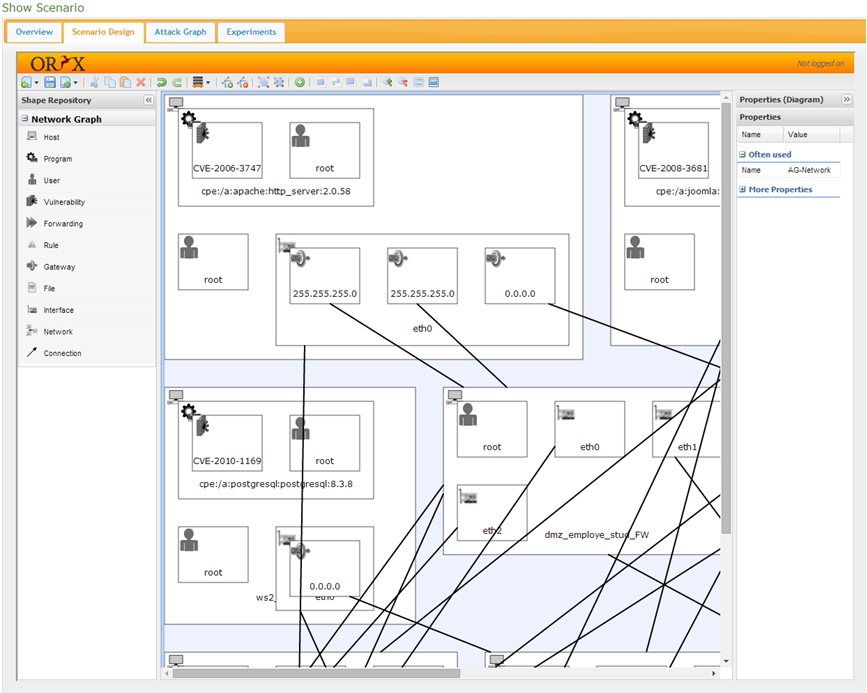
\includegraphics[width=\textwidth]{slg.png}
\caption{SLG}
\label{overflow}
\end{figure}
SLG can be used in multiple use cases, but the main objective to provide a platform for the teaching and study of network security issues. For example, it can be used for Capture The Flag (CTF) seminars.


SLG can be used in multiple use cases, but the main purpose is providing the platform for teaching and researching of network security issues. For example, it could be used for Capture The Flag (CTF) seminars. The idea of the seminar is that the tutor deploys a potentially vulnerable network with vulnerable applications. Students, in turn, are trying to gain access to the network and virtual machines using found vulnerabilities to find flags. The flag is some label or code. The SLG should provide capability not only to deploy the network environment, but also to monitor user activities, find out compromised machines, make a report on ways of hacking the system. But these features do not implemented yet. 
  
  
In the this section we just learned Security Lab Generator. On the next section we will introduce OpenStack technologies and the proposal of migrating SLG on the Cloud as the new project CloudSLG in the section "4.4 Security Lab Generator based on OpenStack". 


 

%The current state of the project does not allow to use it for real seminar. SLG requires %implementation of some necessary features. 





%\end{document} 